%        File: report.tex
%     Created: Sun Oct 22 12:00 AM 2017 C
% Last Change: Sun Oct 22 12:00 AM 2017 C
%

\documentclass[11pt]{article}

\title{FP-Growth Report}
\date{\today}
\author{Trevor Steil}

\usepackage{amsmath}
\usepackage{amsthm}
\usepackage{amssymb}
\usepackage[margin=1.0in]{geometry}
\usepackage{esint}
\usepackage{enumitem}
\usepackage{algorithm}
\usepackage{algorithmicx}
\usepackage{algpseudocode}
\usepackage{bbm}
\usepackage{xcolor}
\usepackage{subcaption}
\usepackage{graphicx}

\newtheorem{theorem}{Theorem}[section]
\newtheorem{corollary}{Corollary}[section]
\newtheorem{proposition}{Proposition}[section]
\newtheorem{lemma}{Lemma}[section]
\newtheorem*{claim}{Claim}
%\newtheorem*{problem}{Problem}
%\newtheorem*{lemma}{Lemma}
\newtheorem{definition}{Definition}[section]

\newcommand{\R}{\mathbb{R}}
\newcommand{\N}{\mathbb{N}}
\newcommand{\C}{\mathbb{C}}
\newcommand{\Z}{\mathbb{Z}}
\newcommand{\Q}{\mathbb{Q}}
\newcommand{\E}{\mathbb{E}}
\newcommand{\supp}[1]{\mathop{\mathrm{supp}}\left(#1\right)}
\newcommand{\lip}[1]{\mathop{\mathrm{Lip}}\left(#1\right)}
\newcommand{\curl}{\mathrm{curl}}
\newcommand{\la}{\left \langle}
\newcommand{\ra}{\right \rangle}
\renewcommand{\vec}[1]{\mathbf{#1}}
\renewcommand{\div}{\mathrm{div}}

\newenvironment{problem}{\textbf{Problem.}}

\newenvironment{solution}[1][]{\emph{Solution #1}}

\algnewcommand{\Or}{\textbf{ or }}
\algnewcommand{\And}{\textbf{ or }}

% Indent paragraphs and remove spacing between paragraphs in itemize and enumerate environments
\setlist{ listparindent=\parindent, parsep=0pt,}


\begin{document}
\maketitle

\section{Implementation}
The FP-Growth algorithm stores a transaction database in a compressed format known as an FP-tree. The FP-tree can be used to
create conditional FP-trees which are essentially projections of FP-trees onto suffix patterns. This allows a recursive approach to frequent itemset
discovery based on growing suffixes contained in itemsets. This method traverses the itemset lattice in a depth-first fashion. We outline some of the
details of implementing this approach below without discussing the details of the algorithm itself.

When creating a conditional FP-tree based on the item $i$, the prefix tree for item $i$ which contains all paths from the root to nodes containing $i$
must be constructed. This is accomplished by following the item pointers between all nodes containing $i$ and copying nodes along the path to the
root. The fact that this tree must be copied in a bottom-up fashion means care must be taken to not copy paths multiple times. If pointers between
nodes containing $i$ are created in order according to the traversal of the itemset lattice, this can be accomplished by keeping track of the last
node containing each item with an ID less than $i$ during the copying of the subtree.

After creating prefix paths containing $i$, the counts stored at nodes must be updated. This can be accomplished by copying counts for nodes
containing $i$ during the creation of prefix paths, setting all other counts to 0, and then propagating these counts up the tree ``level-by-level'', that is, by following the item
pointers for each item with an ID less than or equal to $i$ and adding the count at a node to its parent's count. Updating counts cannot be
effectively performed while creating the prefix paths without repeatedly traversing the same nodes in the FP-tree. For this reason, it is best to
handle counts by traversing the prefix paths once in the fashion outlined.

After updating counts along the prefix paths, the conditional FP-tree can be finished by removing all nodes corresponding to infrequent items and
removing nodes containing the item $i$. These operations only require following pointers between nodes with the same item to count total occurrences
of an item and updating pointers to remove nodes of infrequent items.

Once the conditional FP-tree has been constructed, all remaining items in the tree can be added to the current suffix to give a frequent itemset.
These itemsets can be grown by recursively constructing conditional FP-trees starting from the current FP-tree.

Following the generation of frequent itemsets, rules must be generated. This process can be done using the standard approach of Apriori. In this
approach, supports of needed itemsets have all been computed as these itemsets are all frequent. As this is the case, we can simply store the support
counts for frequent itemsets as they are discovered and search for them during rule generation. Given the order the itemset lattice is explored, we
can store frequent itemsets in a compressed sparse row array and perform a binary search to find frequent itemsets when the support is needed for
computing the confidence of a rule.

\section{Results}

Figure \ref{fig:freq} gives the time required for generating frequent itemsets and number of frequent itemsets generated using the large dataset. At
low support levels, we see very large increases in the number of frequent itemsets generated. The large increase in number of frequent itemsets is
accompanied by a substantial increase in running time. An analysis of this relation was not performed, but from figures \ref{fig:freq_time} and
\ref{fig:freq_count}, the running time appears to possibly be related linearly to the number of itemsets generated.

\begin{figure}[h!]
  \centering
  \begin{subfigure}[t]{0.45\textwidth}
    \centering
    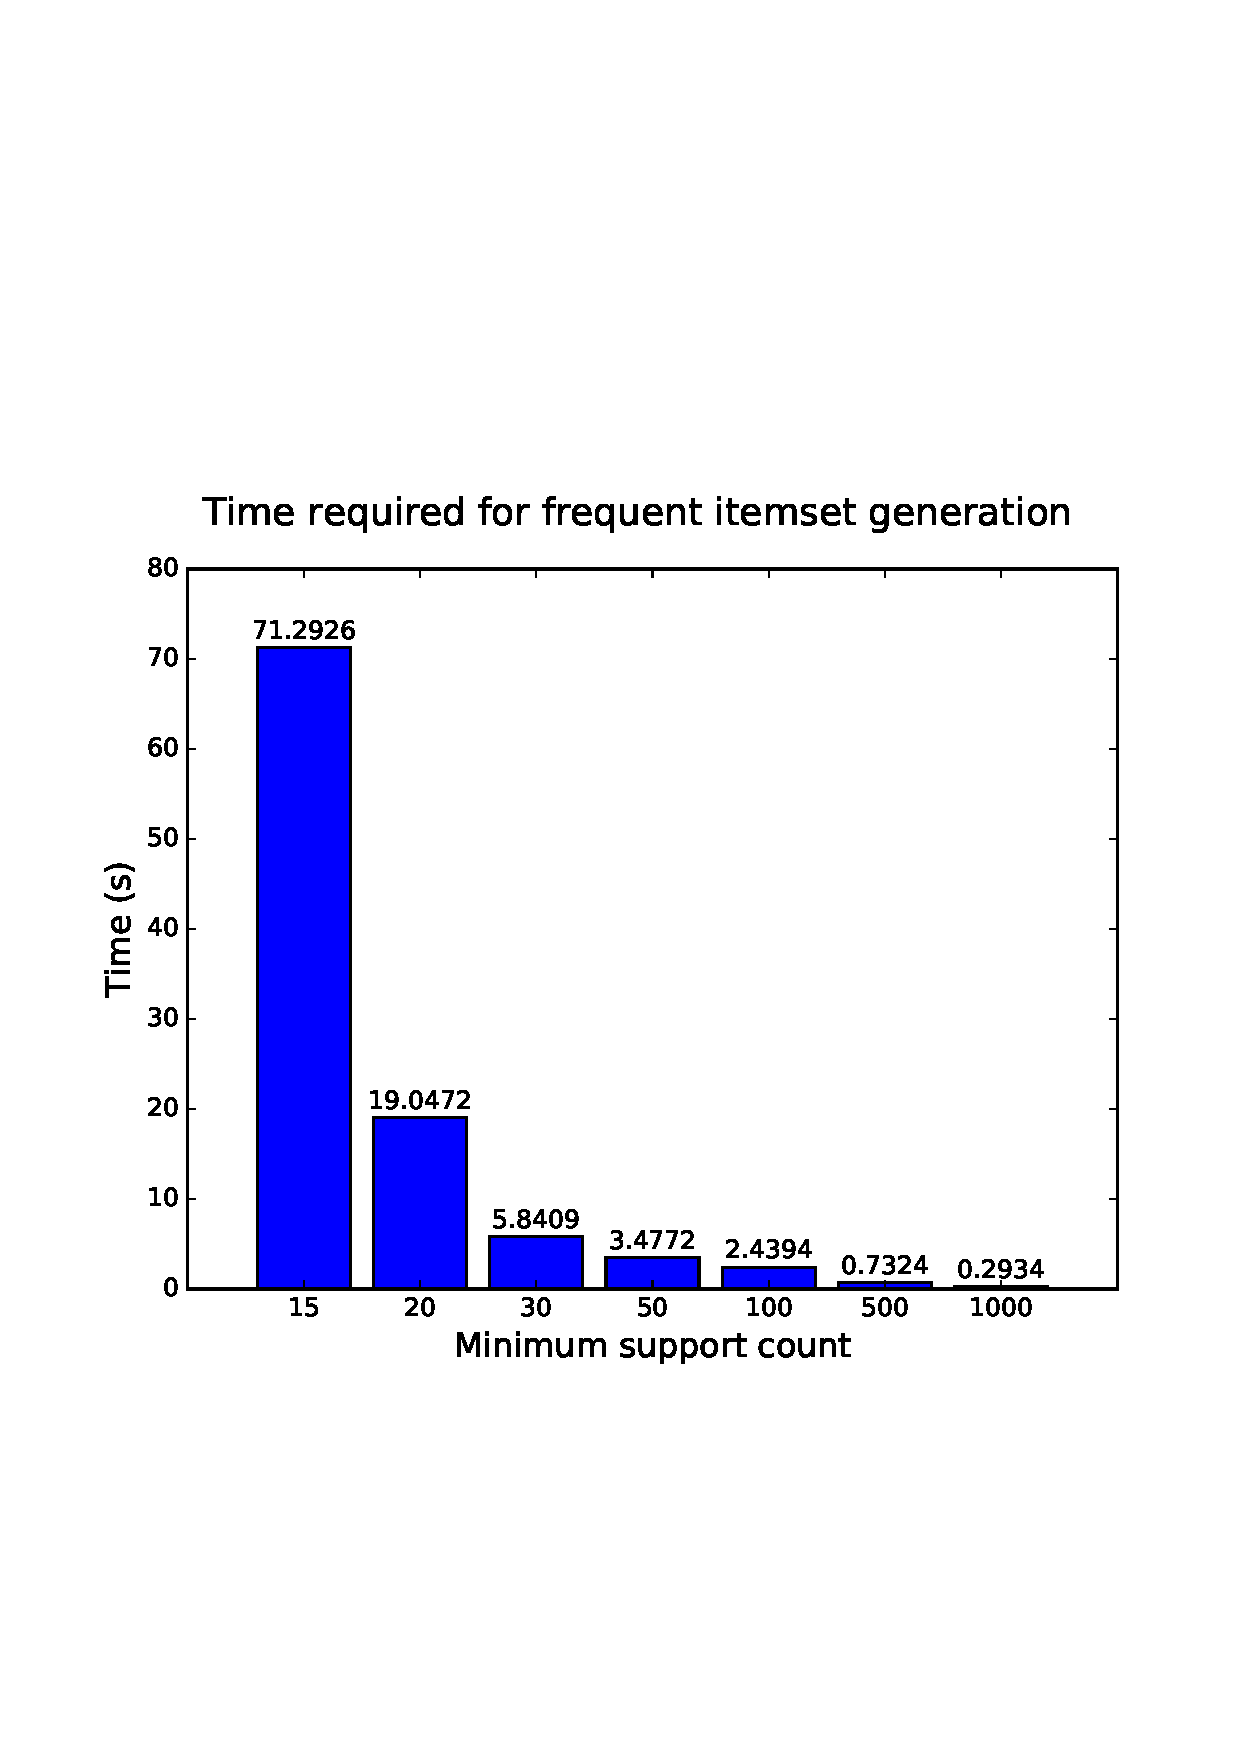
\includegraphics[height=2in]{freq_time.pdf}
    \caption{Time for frequent itemset generation with various minimum support counts}
    \label{fig:freq_time}
  \end{subfigure}
  \begin{subfigure}[t]{0.45\textwidth}
    \centering
    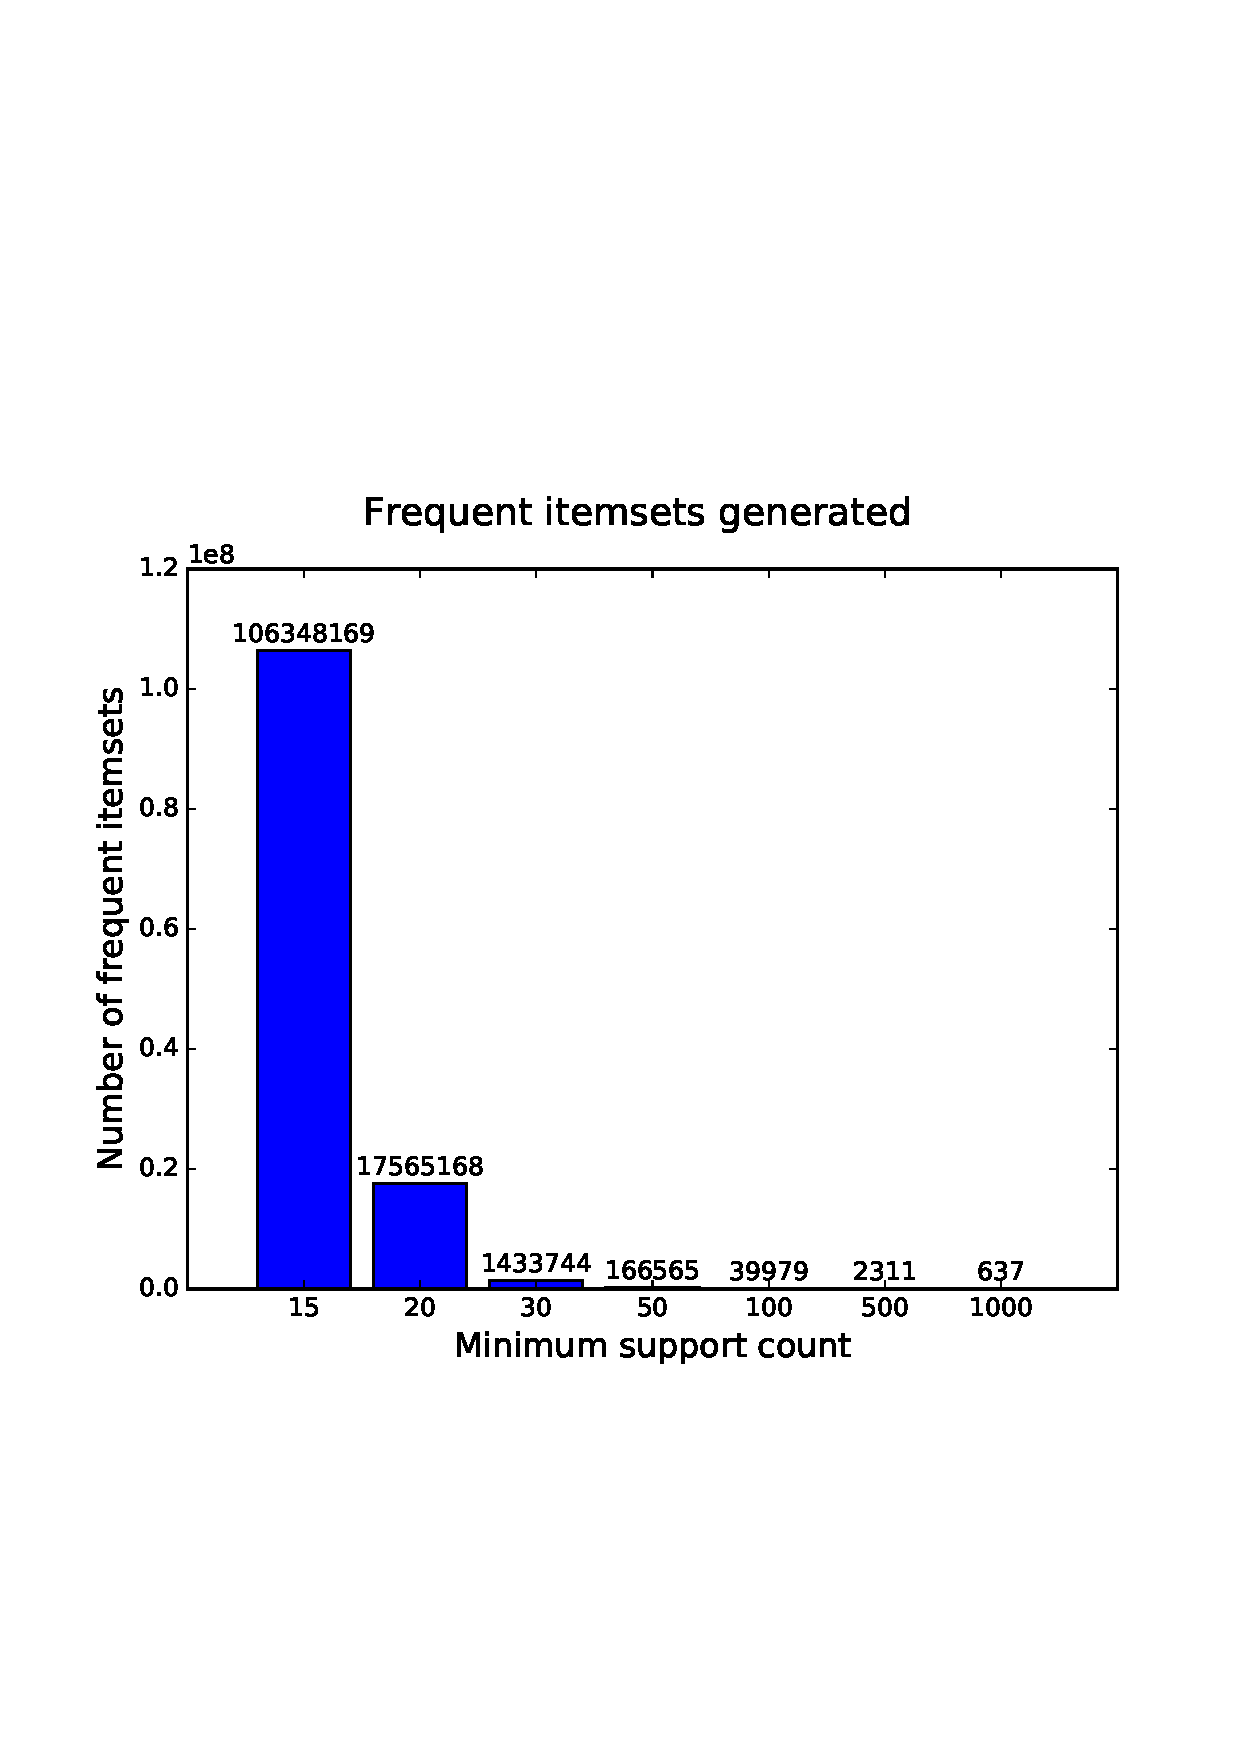
\includegraphics[height=2in]{freq_count.pdf}
    \caption{Number of frequent itemsets generated with various minimum support counts}
    \label{fig:freq_count}
  \end{subfigure}
  \caption{Frequent itemset generation with various minimum support counts}
  \label{fig:freq}
\end{figure}

Figure \ref{fig:rule} gives the time required for generating rules and the number of rules generated from the large dataset for various minimum
confidence levels using a minimum support of 50. Comparing the times corresponding to a minimum support count of 50 in figure \ref{fig:freq_time}, we
see from figure \ref{fig:rule_time} that rule generation time was a small fraction of the time required for frequent itemset discovery, as we expected to
see.

The relation between running time and number of rules generated is slightly harder to identify for rule generation given the smaller number of data points
and the large number of frequent itemsets that need to be processed relative to the number of rules generated. In this case, we see that there
are between 82000 and 422000 rules generated for these minimum confidence levels. Looking in figure \ref{fig:freq_count}, there are approximately
167000 frequent itemsets that need to be processed during rule generation. Much of the running time for rule generation may be due to the large number
of frequent itemsets that need to be processed relative to the number of rules generated, causing running times to be closer together than the number
of rules for different confidence levels. A more useful measure for trying to explain differences in running times would probably be the total number
of candidate rules at each confidence level.

\begin{figure}[h!]
  \centering
  \begin{subfigure}[t]{0.45\textwidth}
    \centering
    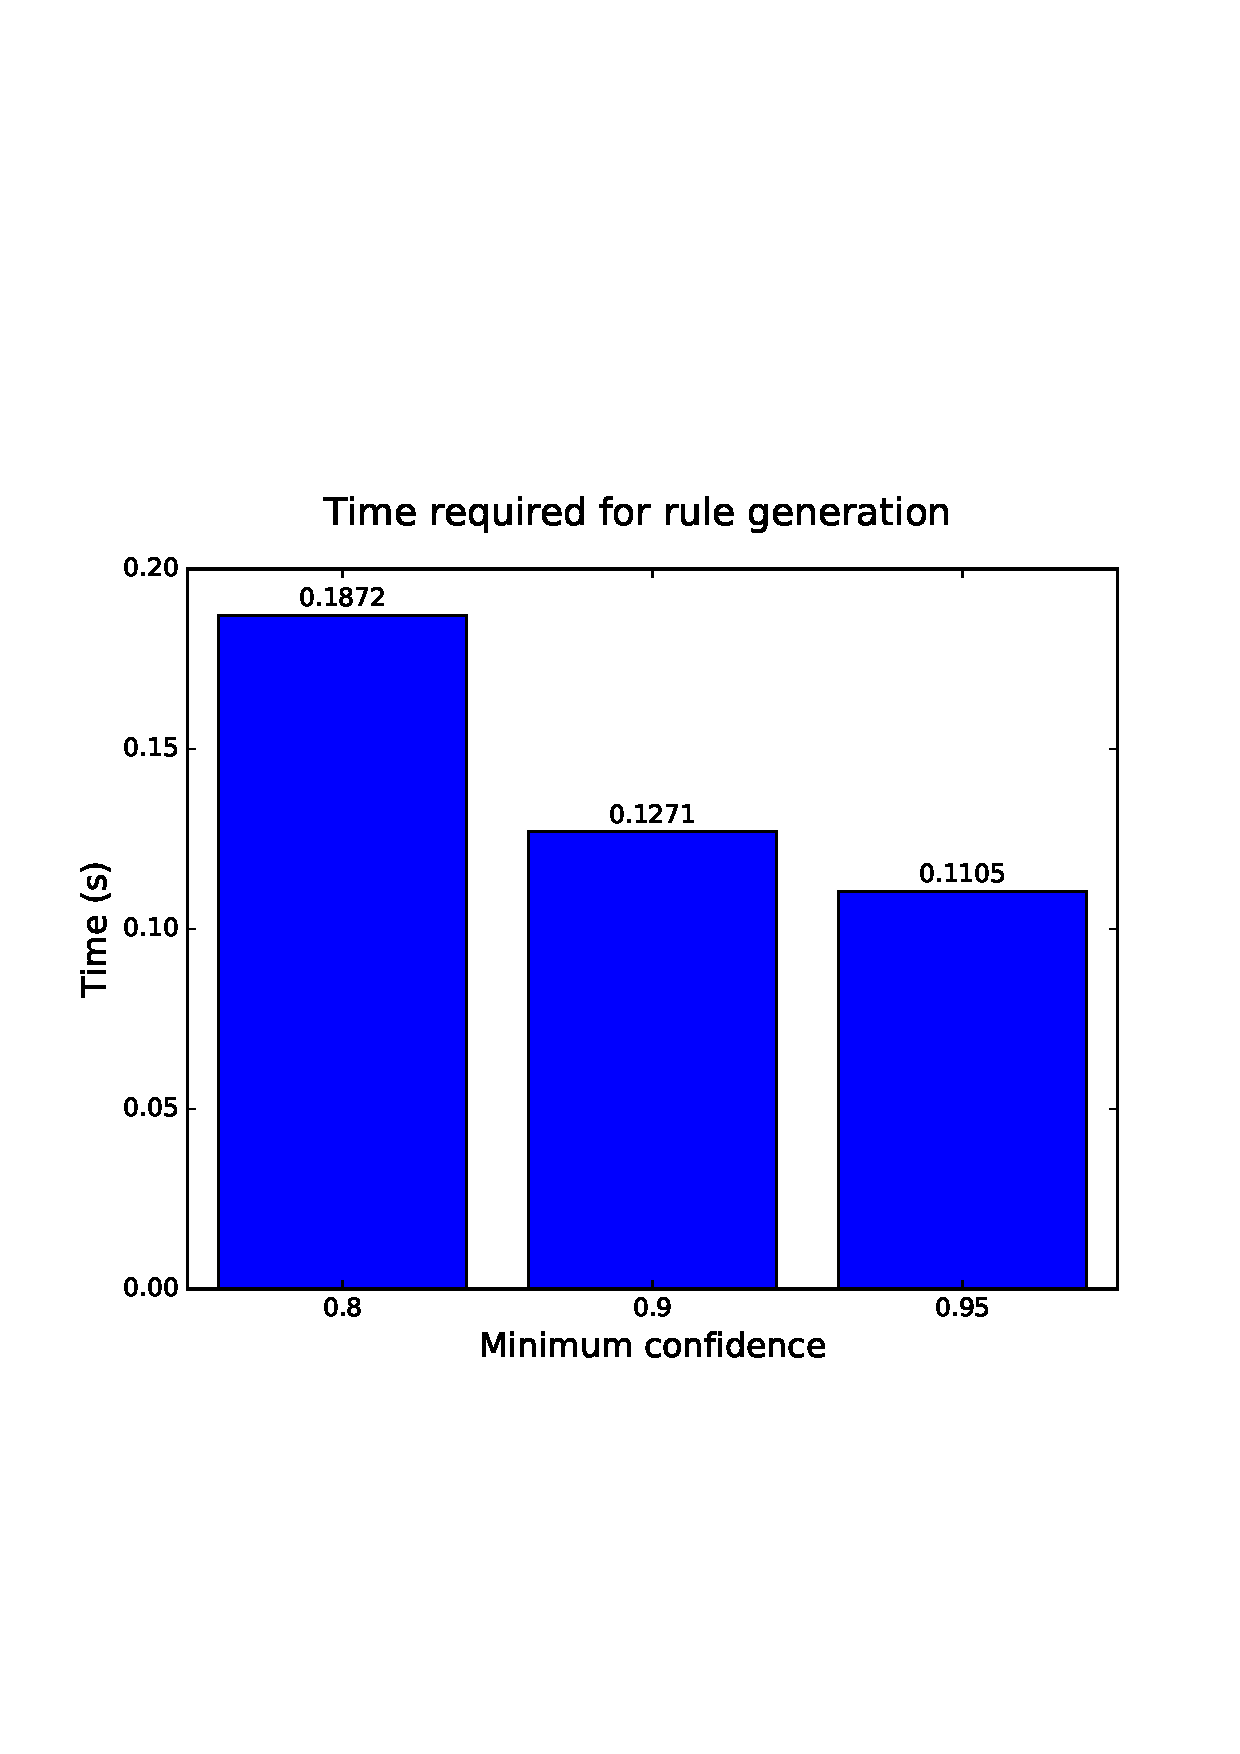
\includegraphics[height=2in]{rule_time.pdf}
    \caption{Time for frequent itemset generation with various minimum confidence levels with a minimum support count of 50}
    \label{fig:rule_time}
  \end{subfigure}
  \begin{subfigure}[t]{0.45\textwidth}
    \centering
    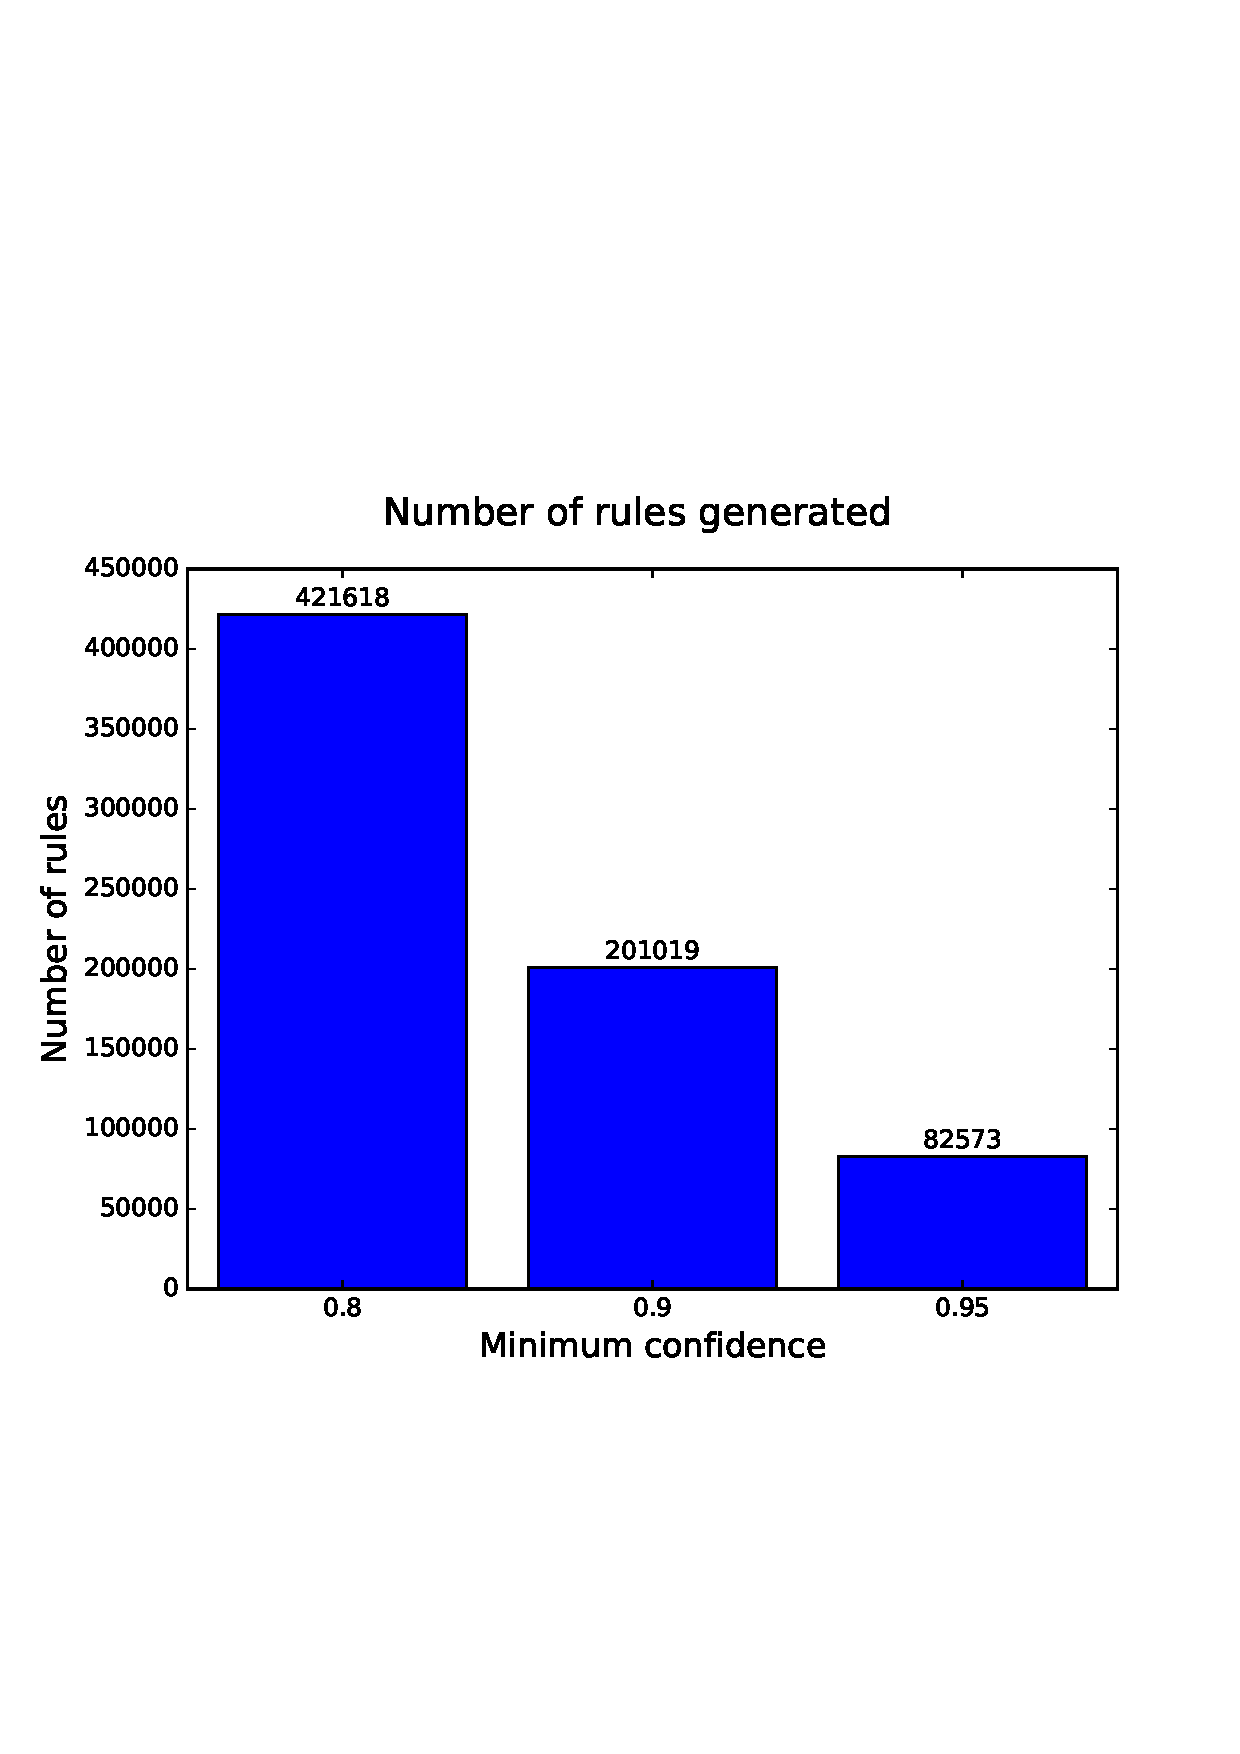
\includegraphics[height=2in]{rule_count.pdf}
    \caption{Number of rules generated with various minimum confidence levels with a minimum support count of 50}
    \label{fig:rule_count}
  \end{subfigure}
  \caption{Rule generation with various minimum confidence levels and a minimum support count of 50}
  \label{fig:rule}
\end{figure}

\section{Further Improvements}
From this project there are a few improvements that could probably lead to improved performance. First, we notice that completely linear conditional
FP-trees can have frequent itemsets extracted more easily. Each further conditional FP-tree constructed from a linear FP-tree will also be linear, so
instead of explicitly constructing further conditional FP-trees, the frequent itemsets can be found by following the path from the root until a node
is found with an insufficient support count. Every frequent itemset in this conditional tree corresponds to a combination of items at nodes above this
point in the tree.

The above observation can be used to generate frequent itemsets deep in the FP-tree. The standard recursive algorithm can be used to generate frequent
itemsets until the conditional FP-tree is linear, at which point the suffix can be grown by taking all combinations of items at nodes with a support
count above the threshold.

I made an attempt at using this observation but was unable to get an increase in performance. This is due to the method by which I was checking for
linearity of FP-trees. I was checking after construction of the tree rather than recognizing that I can simply report if a conditional FP-tree is
linear by checking if there is only one node from which the prefix paths are constructed. This change may give a slight increase in performance if
implemented correctly.

Another possibility for improvement would be in the searching of support counts for frequent itemsets during rule generation. I recognized there is an
order in which frequent itemsets are generated that allows for a binary search to be used. Performing a single search in this manner is a $O(\log n)$
operation where $n$ is the number of frequent itemsets generated. The largest value of $n$ we had to generate rules for gave approximately 1.4 million
frequent itemsets. This gives $\log n \approx 20$, which is relatively small. Another approach to this part of the process would be to create a hash
structure to store support counts of frequent itemsets in. I did not investigate this approach because of my lack of familiarity with creating hash
structures, but if the constants involved were small enough, this change could improve the speed of rule generation. This improvement was deemed not
worth further investigation because the computation time was dominated by frequent itemset discovery, not rule generation.

One possible consideration to improve performance would be to look at more effective uses of cache. Given the unstructured
nature of FP-trees, no attempt was made to write code that made efficient use of caching. In this case, we do not have a nice array of data that
obviously lends itself to cache tiling, but there may still be possible improvements from effectively using cache. Beyond these improvements given
above, there are certainly many improvements that were not considered during this project.

\end{document}


